\let\negmedspace\undefined
\let\negthickspace\undefined
\documentclass[journal]{IEEEtran}
\usepackage[a5paper, margin=10mm, onecolumn]{geometry}
%\usepackage{lmodern} % Uncomment if needed for pdflatex
\usepackage{tfrupee} % Include tfrupee package

\setlength{\headheight}{1cm} % Set the height of the header box
\setlength{\headsep}{0mm}     % Set the distance between the header box and the top of the text

\usepackage{gvv-book}
\usepackage{gvv}
\usepackage{cite}
\usepackage{amsmath,amssymb,amsfonts,amsthm}
\usepackage{algorithmic}
\usepackage{graphicx}
\usepackage{textcomp}
\usepackage{xcolor}
\usepackage{txfonts}
\usepackage{listings}
\usepackage{enumitem}
\usepackage{mathtools}
\usepackage{gensymb}
\usepackage{comment}
\usepackage[breaklinks=true]{hyperref}
\usepackage{tkz-euclide} 
\usepackage{listings}
%\usepackage{gvv}                                        
\def\inputGnumericTable{}                                 
\usepackage[latin1]{inputenc}                                
\usepackage{color}                                            
\usepackage{array}                                            
\usepackage{longtable}                                       
\usepackage{calc}                                             
\usepackage{multirow}                                         
\usepackage{hhline}                                           
\usepackage{ifthen}                                           
\usepackage{lscape}
\usepackage{tikz}
\usepackage{circuitikz}
\usepackage{standalone} % For including external TikZ files

\begin{document}

\bibliographystyle{IEEEtran}
\vspace{3cm}

\title{9.6.7}
\author{EE24BTECH11066 - YERRA AKHILESH}
% \maketitle
% \newpage
% \bigskip
{\let\newpage\relax\maketitle}

\renewcommand{\thefigure}{\theenumi}
\renewcommand{\thetable}{\theenumi}
\setlength{\intextsep}{10pt} % Space between text and floats

\numberwithin{equation}{enumi}
\numberwithin{figure}{enumi}
\renewcommand{\thetable}{\theenumi}
\textbf{Question}:\\
Find the general solution for the given differential equation.\\
$$x \log x \cdot \frac{dy}{dx} + y = \frac{2}{x} \log x$$\\
\textbf{Solution: }
Divide the given Differential equation by $x \log x$,

\begin{align}
    \frac{dy}{dx} + \brak{\frac{1}{x \log x}} \cdot y = \frac{2}{x^2}
\end{align}

Above Differential equation is of form \textbf{first-order linear differential equation} and its general form is expressed as:
\begin{align}
    \frac{dy}{dx} + P(x) \cdot y = Q(x)
\end{align}
and the general solution is,
\begin{align}
    \mu \brak{x} \cdot y = \int \mu \brak{x} Q(x) \, dt
\end{align}
where $\mu \brak{x}$ is an integrating factor, expressed as 
\begin{align}
\mu \brak{x} = e ^ {\int P(x) \, dx}
\end{align}
for the given question,
\begin{align}
    \mu \brak{x} = e ^ {\int \frac{1}{x \log x} \, dx} \\
    \log x = t 
\end{align}
Differentiate with x on both sides,
\begin{align}
    \frac{1}{x} \cdot dx = dt
\end{align}
Therefore $\mu \brak{x}:$
\begin{align}
    \mu \brak{x} = e ^ {\int \frac{1}{t} \, dt}\\
    \mu \brak{x} = e ^ {\log t}\\
    \mu \brak{x} = t = \log x
\end{align}
Substitute this integrating factor in general solution,
\begin{align}
    y \cdot \log x = \int \log x \cdot \frac{2}{x^2} \, dx
\end{align}
Integrate the right-side part using by-parts,
\begin{align}
    y \cdot \log x = 2 \brak{\brak{\log x \cdot \int {\frac{1}{x^2}} \, dx} + \brak{\int \frac{1}{x^2}\, dx}}\\
    y \cdot \log x = 2 \brak{\log x \cdot \frac{x^{-1}}{-1} - \frac{1}{x}} + c\\
    y \cdot \log x = -2 \cdot \frac{\log x}{x} - \frac{2}{x} +c 
\end{align}
Divide with $\log x$ on the both sides and assume $c = 0$,
\begin{align}
    y(x) = \frac{-2}{x} \brak{1 + \frac{1}{\log x}}
\end{align}
Now let us verify this computationally
From definition of $\frac{dy}{dx}$,
\begin{align}
    y_{n+1}=y_{n}+\frac{dy}{dx}\cdot h
    \label{0.15}
\end{align}
(where h is small number tending to zero)
From the differential equation given,
\begin{align}
    \frac{dy}{dx}=\frac{2}{x ^ 2} -  \frac{y}{x \log x}
    \label{0.16}
\end{align}
By substituting,
\begin{align}
    y_{n+1}=y_{n}+\brak{\frac{2}{x_n ^ {2}} - \frac{y_n}{x_n \log {x_n}}}\cdot h
\end{align}
By taking $x_1=0.1 \text{ and } y_1=-11.32$  and $h=0.001$ going till $x=1$ by iterating through the loop and finding $y_2,y_3,\cdots , y_{500}$ and plotting the graph, we can verify if the function we got by solving the differential equation mathematically.
\begin{figure}[H]
    \centering
    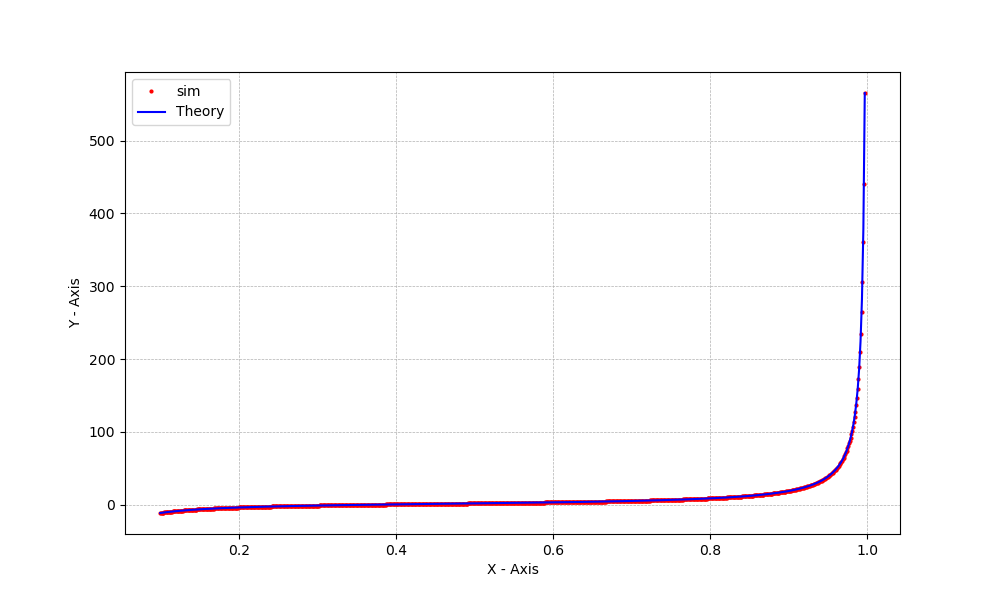
\includegraphics[width = \columnwidth]{figs/Figure_1.png}
\end{figure}
\end{document}
